\section{Task 3: \\ Implementation of Iterative Deepening}
The goal of this task was to implement iterative deepening and use it in a second phase to adjust our program to be able to handle time limits.\\
For this we will execute the move search multiple, while each time increasing the search depth, starting at 1.\\
Due to the exponential growth of game trees, we do not loose too much time by regenerating the trees of smaller depth again and again.\\\\
For an average branching factor of $b$ and depth $d$, we can calculate the average amount of nodes:\\
\begin{center}
	${\displaystyle \sum_{k=1}^{d}(b^{k})} = \frac{b^{d+1}-b}{b-1}$
\end{center}
To execute the move search for depths $1$ to $d-1$, we can determine approximate amount of nodes visited \\
\begin{center}
	${\displaystyle \sum_{k=1}^{d-1}(\frac{b^{k+1}-b}{b-1})} = -\frac{b(-b^{d}+bd-d+1)}{(b-1)^{2}}$
\end{center}
We can now compute the ratio between the nodes in the trees of depth $1$ to $d-1$ and in the tree of depth $d$:
\begin{center}
	${\displaystyle \dfrac{\frac{b^{d+1}-b}{b-1}}{\frac{b^{d+1}-b}{b-1}+(-\frac{b(-b^{d}+bd-d+1)}{(b-1)^{2}})}}$
\end{center}
In the following picture this ratio is visualized. We see that the tree of depth d take a large amount of the time, for bigger trees even more. So we only loose a small fraction of the time to compute the tree for depth $1$ to $d$ in advance.\\

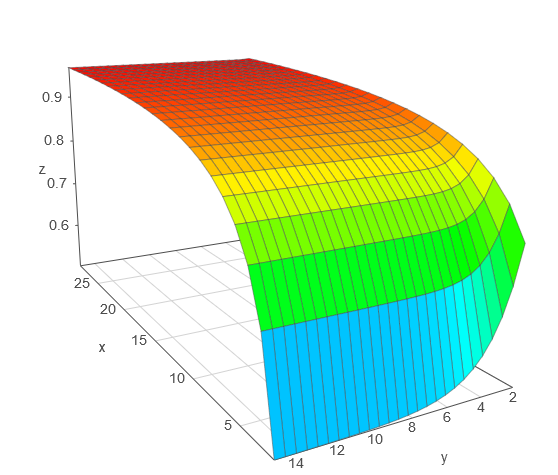
\includegraphics{deepening}

x : stands for the branching factor b

y : stand for the search depth d

z : ratio\\
\color{gray}
All computation were made with WolframAlpha\\
To plot the function we used the tool on the site of academo.org
\color{black}
\\\\
With alpha beta pruning we would not generate all of these nodes, but the proportion would remain the same.\\

By using iterative deepening we have two advantages. The first one is that we can save what moves looked promising in a previous iteration and execute them first. Like this we expect to get the $alpha$ and $beta$ values closer together as they normally would and be able to prune away more of the tree. Effectively approaching the best-case runtime of alpha-beta pruning of $O(b^{d/2})$ (which is reached if we execute the best move first).\\
Further we have the advantage that after the first iteration has finished, we always have move that we can return once the time has run out. So we avoid to return a move after only have analysed a fraction of the board.\\

This leads us to the second part of this task, the capability of reacting to a time limit. 
We achieved this by using the methode call
\begin{lstlisting}[frame=none, numbers=none]
setitimer (ITIMER\_REAL, \&timer, 0).
\end{lstlisting}
The first argument is the type of the timer. Here we use a real-time timer as the server also count in real time. 
The second argument sets the time until the timer sends a signal. The last argument is not needed.\\\\
The timer arguments are set as following (in advance we have already subtracted 50 ms from the search time to account for time it takes to close all the recursion stacks, free the memory and send a message to the server):
\begin{lstlisting}[frame=none, numbers=none]
timer.it\_value.tv\_sec = (searchTime/2)/1000;
timer.it\_value.tv\_usec = (searchTime/2)%1000)*1000;
timer.it\_value.tv\_sec = (searchTime/2)/1000;
timer.it\_value.tv\_usec = (searchTime/2)%1000)*1000;
\end{lstlisting}
The first 2 values define, in seconds and microseconds, when the timer should send a signal the first time. 
With the third and forth argument we set the interval at which the timer should keep firing after the first time. 
Before we leave our move search algorithm, we cancel the timer to make sure it does not go off at an unexpected moment and cause undefined behaviour. This is done by recalling the the setitimer methode with all the timer arguments zeroed.\\

The last step was to write the callback function to define what happens once the timer sends a signal.
As the timer runs in a separate thread when executing the code of the callback function, we have to avoid race conditions. 
To achieve this we use flag of type \textbf{static volatile sig\_atomic\_t}.\\

The first call of the callback function will set the \textbf{hasHalfTimePassed}-flag, the second one the \textbf{hasTimePassed}-flag.
The \textbf{hasHalfTimePassed}-flag is checked after every iteration. If we have less than half our time we can assume that we will not finish the next iteration. SO we will return immediately and save the time for the following turn.
The \textbf{hasTimePassed}-flag is checked constantly during the move search to make sure we will catch it as soon as possible and have enough time to return the move found in the previous iteration.



